\documentclass[a4paper, 12pt]{article}
\usepackage{titling}
\usepackage{array}
\usepackage{booktabs}
\usepackage{enumitem}
\usepackage{graphicx}
\usepackage{hyperref}
\usepackage{amssymb}
\usepackage{listings}
\usepackage{color} %red, green, blue, yellow, cyan, magenta, black, white
\setlength{\heavyrulewidth}{1.5pt}
\setlength{\abovetopsep}{4pt}
\setlength{\parindent}{0pt}
\graphicspath{{.}}

\usepackage[margin=1in]{geometry}
\definecolor{mygreen}{RGB}{28,172,0} % color values Red, Green, Blue
\definecolor{mylilas}{RGB}{170,55,241}
% Must be after geometry
\usepackage{fancyhdr}
\pagestyle{fancy}
\fancyhf{}
\rhead{SEE Assignment 4}
\lhead{P.Lukin, E. Ovchinnikova}
\cfoot{\thepage}

\setlength{\droptitle}{-5em}

\title{Scientific Experimentation and Evaluation  \\
				Assignment: 4}
\author{Petr Lukin, Evgeniya Ovchinnikova}
\date{Lecture date: $24^{th}$ October 2016}

\begin{document}
%-------------------------------------------------------------------------------
\lstset{language=Matlab,%
    %basicstyle=\color{red},
    breaklines=true,%
    morekeywords={matlab2tikz},
    keywordstyle=\color{blue},%
    morekeywords=[2]{1}, keywordstyle=[2]{\color{black}},
    identifierstyle=\color{black},%
    stringstyle=\color{mylilas},
    commentstyle=\color{mygreen},%
    showstringspaces=false,%without this there will be a symbol in the places where there is a space
    numbers=left,%
    numberstyle={\tiny \color{black}},% size of the numbers
    numbersep=9pt, % this defines how far the numbers are from the text
    emph=[1]{break},emphstyle=[1]\color{red}, %some words to emphasise
    %emph=[2]{word1,word2}, emphstyle=[2]{style},
}

%-------------------------------------------------------------------------------


\maketitle

\section{Experiment setup}

The current experiment was conducted using AICISS optical tracking system - three USB-cameras (lifecam19,20,22) mounted on the ceiling in a room C022. The cameras are pre-calibrated, so we didn't need to perform a calibration by ourselves as we did in the previous assignment. For this system usage we needed to install a marker that would be tracked by the system on the robot. We have generated some new markers (Fig. \ref{fig:markers}) and added them and their linear size (10 $\times$ 10 cm) to the dictionary:

\begin{lstlisting}

dictionary.yml:

%YAML:1.0
nmarkers: 5
markersize: 4
marker_0: "0111000111100101"
marker_1: "1100011000010101"
marker_2: "0110101010001001"
marker_3: "0011001000011111"
marker_4: "0101010000111100"

see_robot.json

{
    "Markers":
    {
        "15402":
        [
            "70.0 -70.0",
            "70.0 70.0",
            "-70.0 70.0",
            "-70.0 -70.0"
        ]
    },
    "Dimensions":
    {
        "Length": "100",
        "Width": "100"
    }
}

\end{lstlisting}

\begin{figure}[h]
  \centering
  \caption{Two of newly generated markers.\label{fig:markers}}
  
\includegraphics[width=0.5\textwidth]{markers}
\end{figure}

It is important for the measurement that the marker is well fixed, doesn't shake and is parallel to the floor, so we've made the construction depicted in Fig. \ref{fig:markerHolder} to fix the marker on it.

\begin{figure}[h]
  \centering
  \caption{A marker holding construction.\label{fig:markerHolder}}
  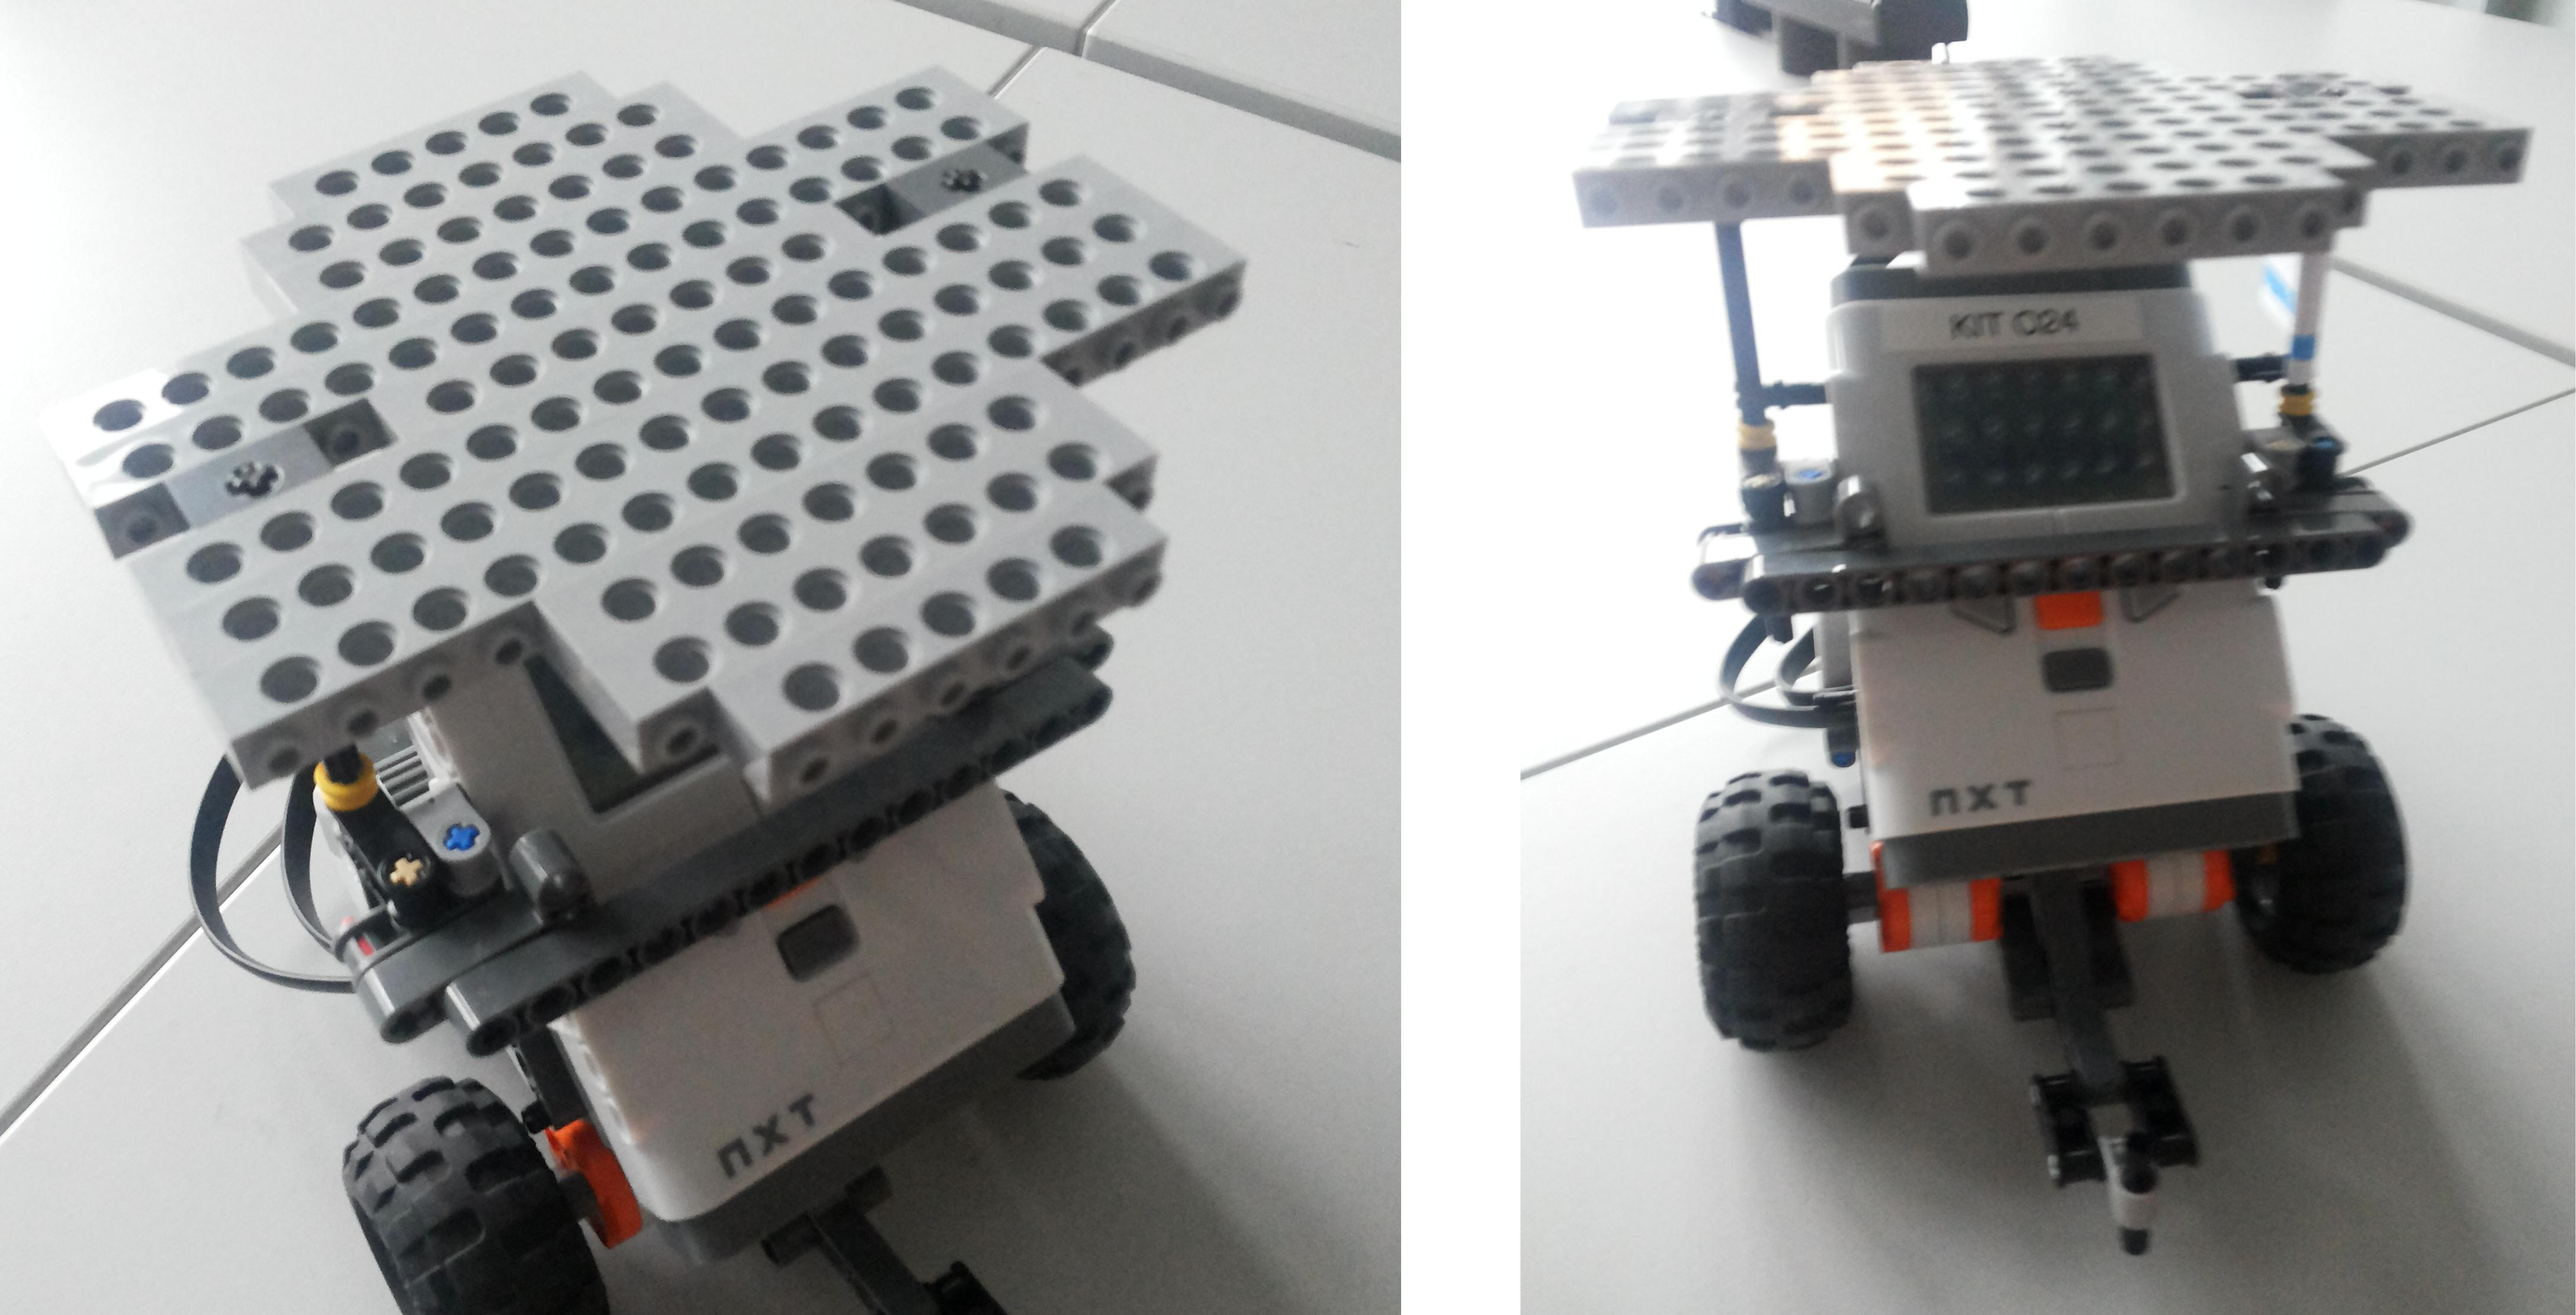
\includegraphics[width=0.5\textwidth]{markerHolder}
\end{figure}

One can see that the platform is wide enough for the marker, so it won't bend and the crossbar in the middle makes it not shaky. It was also placed in such a way so it will be as close as possible with the details we have to the robot's center of the mass so it won't outbalance it. Another important point is that the the markers must have a white frame around it, otherwise it will be detected inaccurately. First time we've tried to conduct an experiment using a wrong marker (Fig. \ref{fig:wrongMarker}) and the results were inacceptable -- in some positions cameras just have lost the robot. Therefore, we have changed the setup to leave some white field and used a smaller size, so it would be easier to mount it so it would be fatter, that one can see in Fig. \ref{fig:rightMarker}. In this case cameras didn't loose the robot in any position in the driving part of the room.

\begin{figure}[h]
  \centering
  \caption{A wrong marker mount.\label{fig:wrongMarker}}
  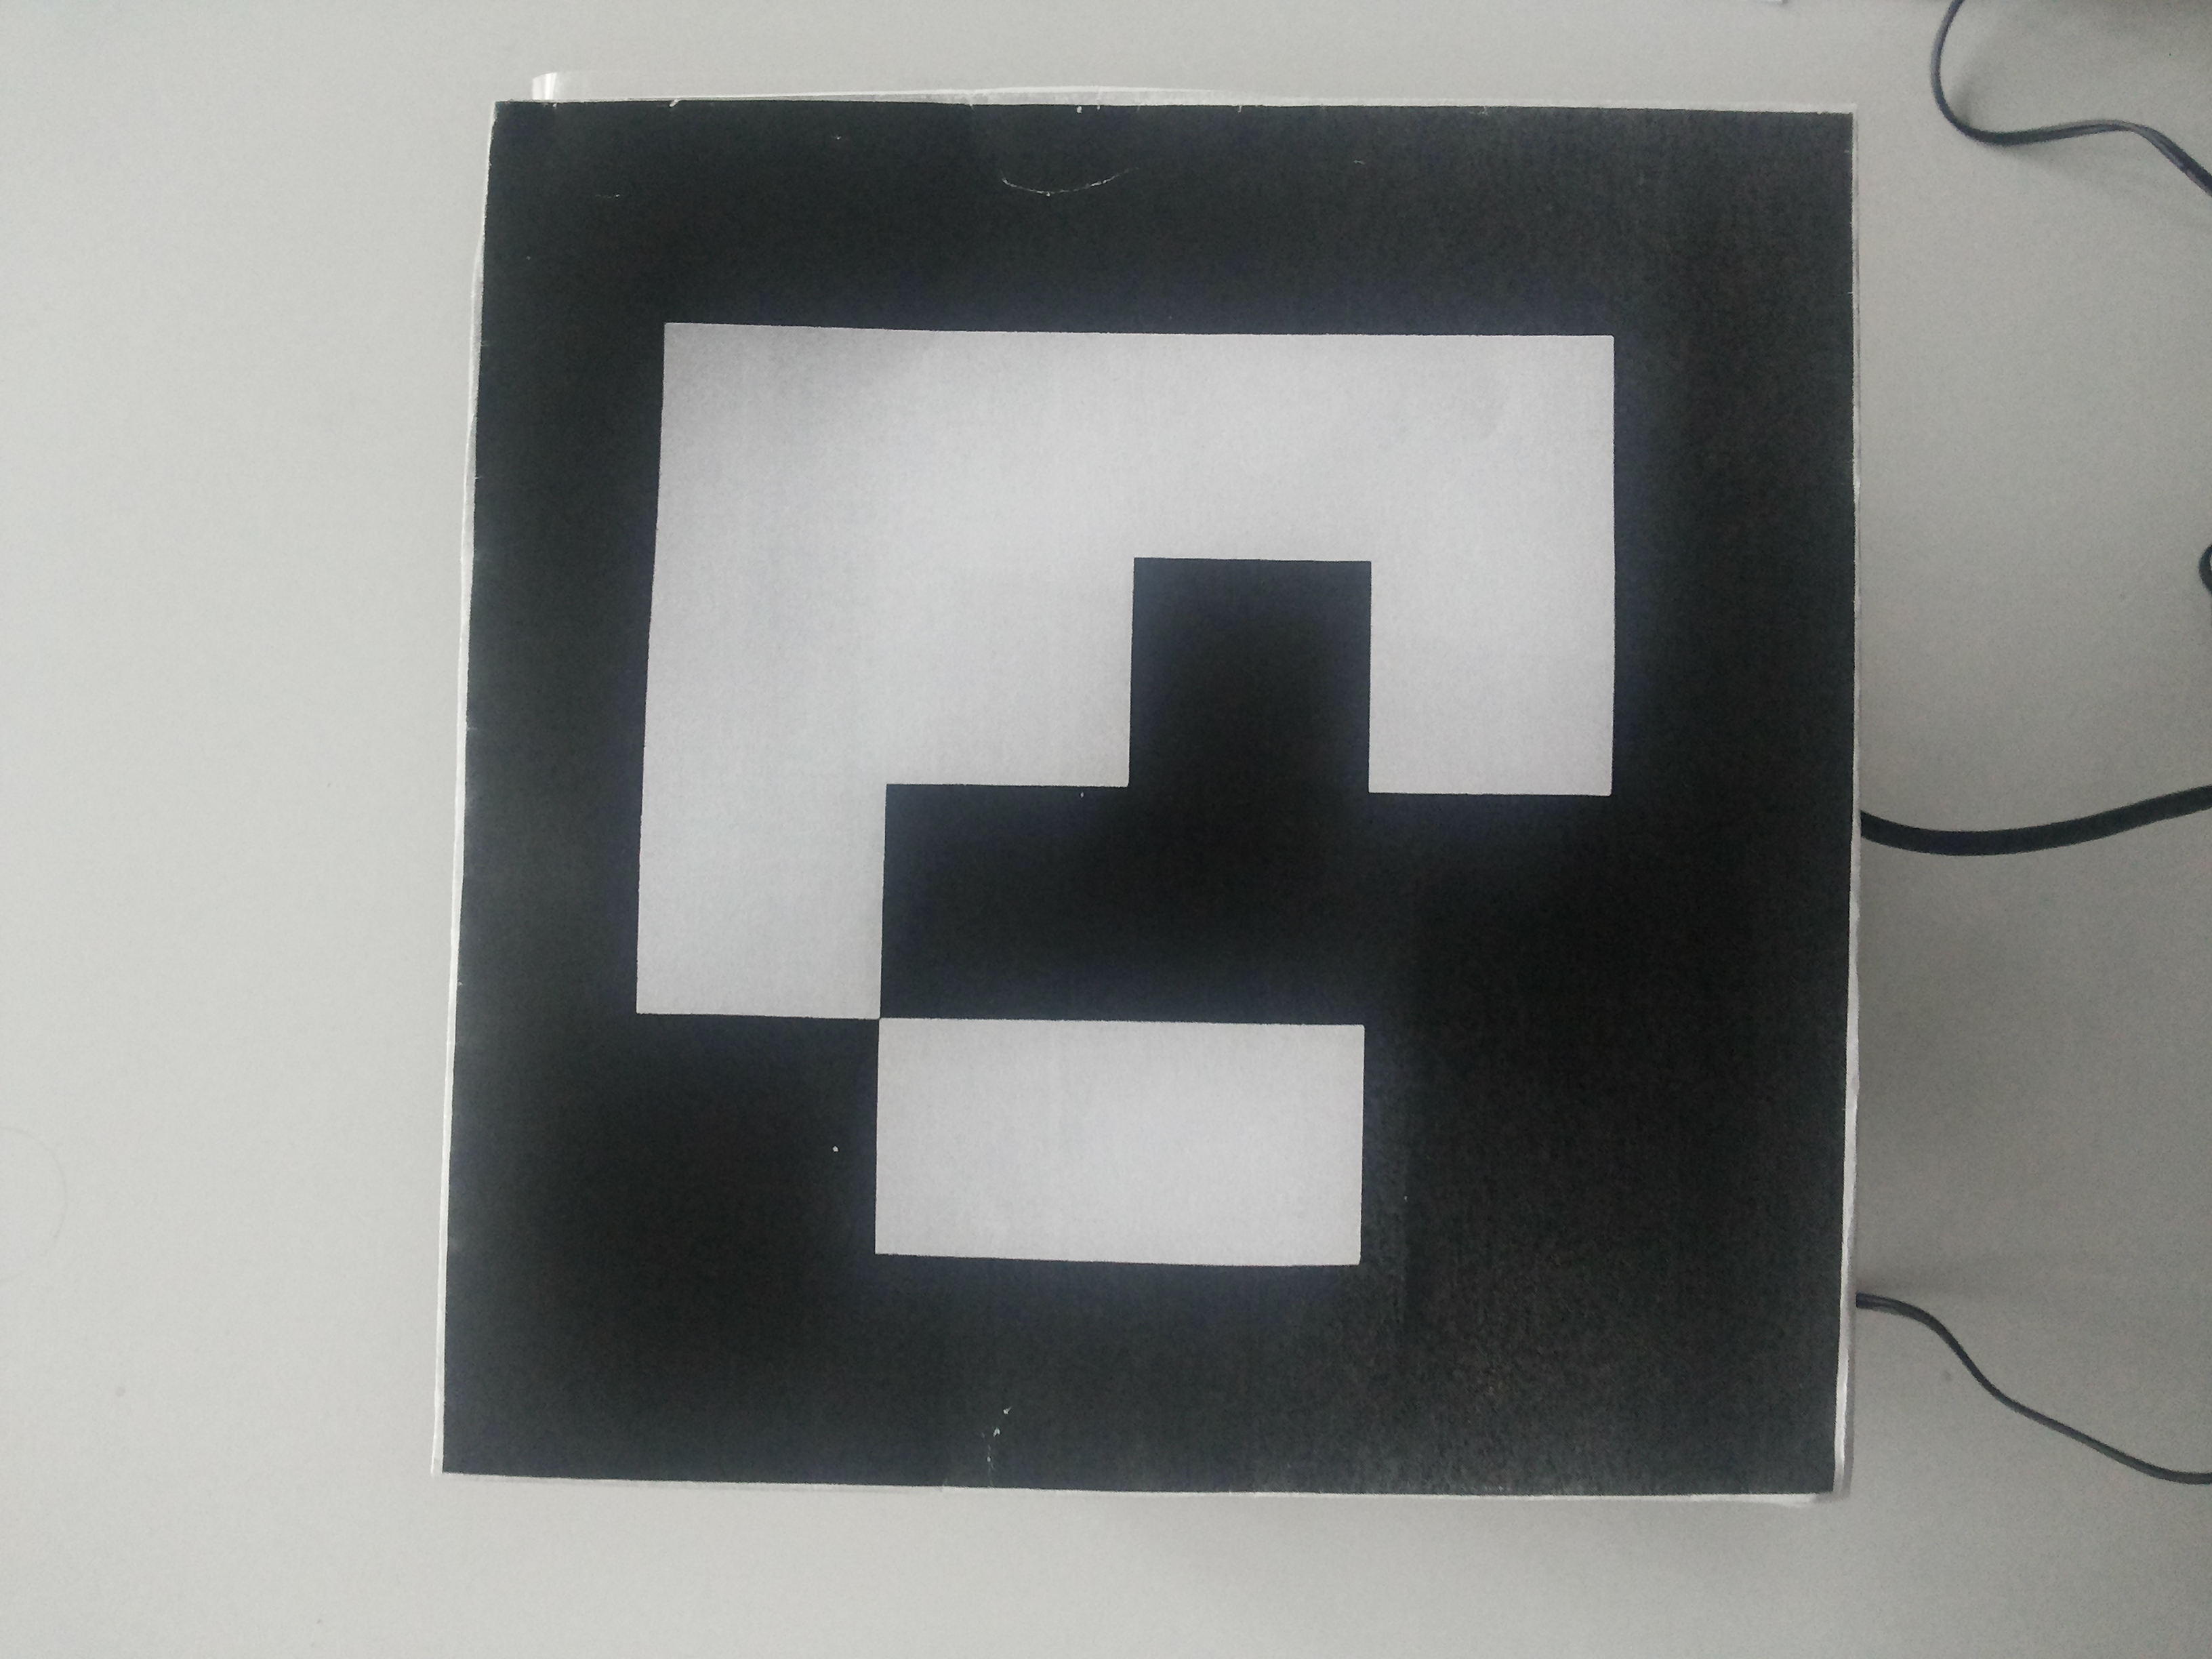
\includegraphics[width=0.3\textwidth]{wrongMarker}
\end{figure}

\begin{figure}[h]
  \centering
  \caption{A correct mount of the marker.\label{fig:rightMarker}}
  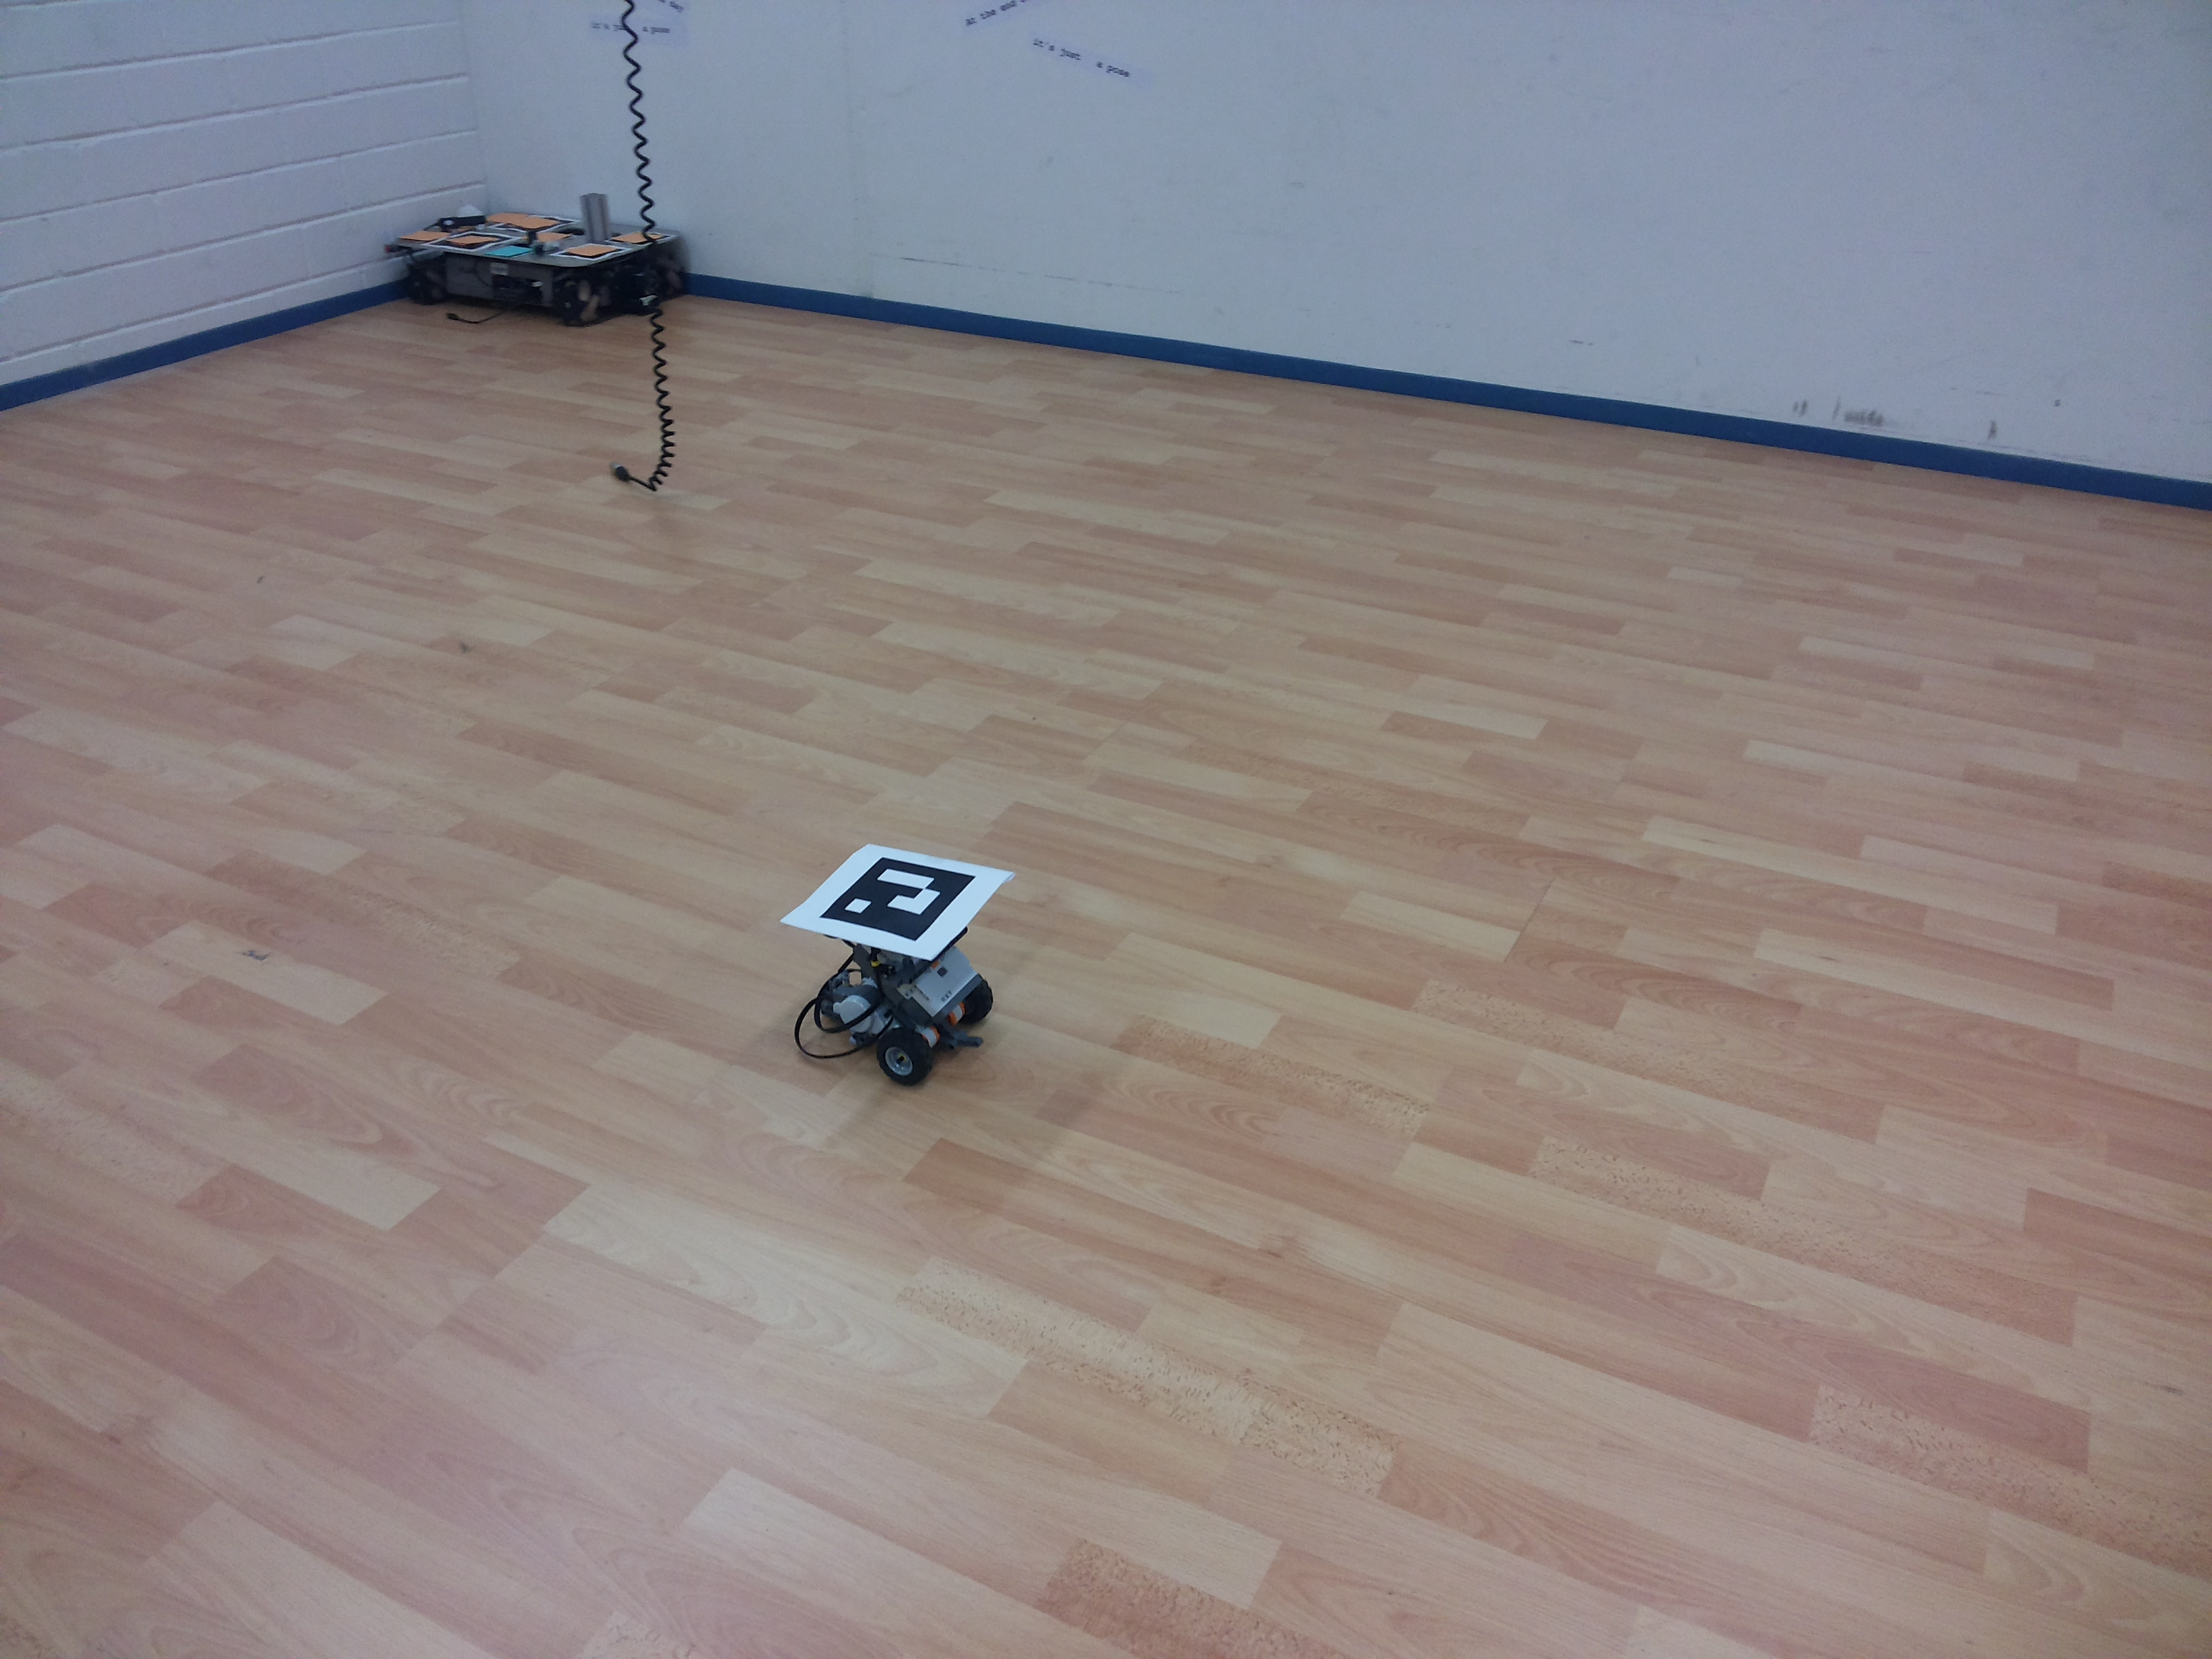
\includegraphics[width=0.5\textwidth]{rightMarker}
\end{figure}

To check if the system is working correctly, we've used a paper and a ruler in a way similar to the previous experiment on short distances, so the robot's motion error won't harm the results. The system was proven to be working correctly, however, the a number of simbols after comma in AICISS's measurement is much larger than we can possibly estimate by hands, so we cannot say anything about the exact precision of the system. \\

There are the following possible pitfalls:
\begin{itemize}
\item imperfections of the robot construction - since we are limited in details, it is hard to make a perfectly unshakable construction. We could not see it visually, but there could be a minor shaking that could affect the precision of the measurement
\item imperfection of robot's motors
\item problems related to a camera switching. To make it smoother we've used a video stitching tool (that can make a one video of three)
\item our robot is too small to mount multiple markers as it is done with youBot, so it has more problems with camera switching. If we would have tried to put more markers it would have either unbalance the system if it would have been on the top or harmed the motion if it would have been following the robot on some additional wheeled platform
\item imperfections of the cameras
\item the experiment took quite a lot of time, so the illumination changed
\item the camera calibration model perhaps not uses the skew (shear distortion), so if there is the one, it may cause the problems
\end{itemize}

\section{Program code}

It is sensible to make the measurements using the same parameters those we used in previous experiment. Construction of the robot wasn't changed much, so we'll be able to make a good comparison of the two ways of measurements. That is why we've left almost the same code, but without any light sensor activation and with the motion in loops. To distinguish different experimental tracks in the end of each loop step we've used a time delay of 5 seconds. So, if the position is not changing for this time, it is the end position of on track and start position of the second one. \\
For straight motion the robot moved eight times straight (approximately the length of the room), turned for  $180^{\circ}$ and went back. For arc motion robot moved clockwise and counterclockwise in two circles of different diameter (50 and 240 cm). We've used the following code:

\begin{lstlisting}

package LegoNXT;

import lejos.nxt.LightSensor;
import lejos.nxt.Motor;
import lejos.nxt.SensorPort;
import lejos.robotics.navigation.DifferentialPilot;
import lejos.robotics.navigation.MoveController;
import lejos.util.Delay;
import lejos.nxt.Button;

public class goStraight {
	public static void main(String[] args) {
		double arcRad = 40;
		double angle = 90;
		double arcLen = Math.PI*2*arcRad*angle/360;
		double trackWidth = 12;
		DifferentialPilot dp = new DifferentialPilot(MoveController.WHEEL_SIZE_NXT1, trackWidth, Motor.B, Motor.C, true);
		Button.RIGHT.waitForPressAndRelease();
		for (int j = 0; j < 5; j++){
			for (int i = 0; i < 8; i++){
				dp.setTravelSpeed(10);
				dp.travel(-arcLen);
				Delay.msDelay(5000);
			}
			dp.rotate(180);
		}
		Button.ESCAPE.waitForPressAndRelease();
	}
}



package LegoNXT;

import lejos.nxt.LightSensor;
import lejos.nxt.Motor;
import lejos.nxt.SensorPort;
import lejos.robotics.navigation.DifferentialPilot;
import lejos.robotics.navigation.MoveController;
import lejos.util.Delay;
import lejos.nxt.Button;

public class goRight {

	public static void main(String[] args) {
		double arcRad = 25;
		double angle = 90;
		double trackWidth = 12;
		DifferentialPilot dp = new DifferentialPilot(MoveController.WHEEL_SIZE_NXT1, trackWidth, Motor.B, Motor.C, true);
		Button.RIGHT.waitForPressAndRelease();
		for (int i = 0; i < 40; i++){
			dp.setTravelSpeed(10);
			dp.arc(arcRad, -angle);
			dp.stop();
			Delay.msDelay(5000);
		}
		Button.ESCAPE.waitForPressAndRelease();
	}
}


package LegoNXT;

import lejos.nxt.Motor;
import lejos.nxt.SensorPort;
import lejos.robotics.navigation.DifferentialPilot;
import lejos.robotics.navigation.MoveController;
import lejos.util.Delay;
import lejos.nxt.LightSensor;
import lejos.nxt.Button;

public class goLeft {

	public static void main(String[] args) {
		double arcRad = 25;
		double angle = 90;
		double trackWidth = 12;
		DifferentialPilot dp = new DifferentialPilot(MoveController.WHEEL_SIZE_NXT1, trackWidth, Motor.B, Motor.C, true);
		Button.RIGHT.waitForPressAndRelease();
		for (int i = 0; i < 40; i++){
			dp.setTravelSpeed(10);
			dp.arc(-arcRad, angle);
			dp.stop();
			Delay.msDelay(5000);
		}
		Button.ESCAPE.waitForPressAndRelease();
	}
}


package LegoNXT;

import lejos.nxt.Motor;
import lejos.nxt.SensorPort;
import lejos.robotics.navigation.DifferentialPilot;
import lejos.robotics.navigation.MoveController;
import lejos.util.Delay;
import lejos.nxt.LightSensor;
import lejos.nxt.Button;

public class goSlightlyRight {

	public static void main(String[] args) {
		double arcRad = 120;
		double angle = 30;
		double trackWidth = 12;
		DifferentialPilot dp = new DifferentialPilot(MoveController.WHEEL_SIZE_NXT1, trackWidth, Motor.B, Motor.C, true);
		Button.RIGHT.waitForPressAndRelease();
		for (int i = 0; i < 40; i++){
			dp.setTravelSpeed(10);
			dp.arc(arcRad, -angle);
			dp.stop();
			Delay.msDelay(5000);
		}
		Button.ESCAPE.waitForPressAndRelease();
	}
}


package LegoNXT;

import lejos.nxt.Button;
import lejos.nxt.LightSensor;
import lejos.nxt.Motor;
import lejos.nxt.SensorPort;
import lejos.robotics.navigation.DifferentialPilot;
import lejos.robotics.navigation.MoveController;
import lejos.util.Delay;

public class goSlightlyLeft {
	public static void main(String[] args) {
		double arcRad = 120;
		double angle = 30;
		double trackWidth = 12;
		DifferentialPilot dp = new DifferentialPilot(MoveController.WHEEL_SIZE_NXT1, trackWidth, Motor.B, Motor.C, true);
		Button.RIGHT.waitForPressAndRelease();
		
		for (int i = 0; i < 40; i++){
			dp.setTravelSpeed(10);
			dp.arc(-arcRad, angle);
			dp.stop();
			Delay.msDelay(5000);
		}
		Button.ESCAPE.waitForPressAndRelease();
	}
}



\end{lstlisting}
\newpage
\section{Experimental results}

We've obtained the following trajectories:
\begin{center}
  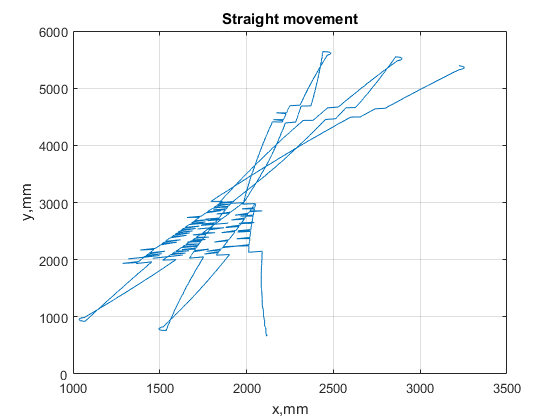
\includegraphics[scale = 0.8]{s.png}

  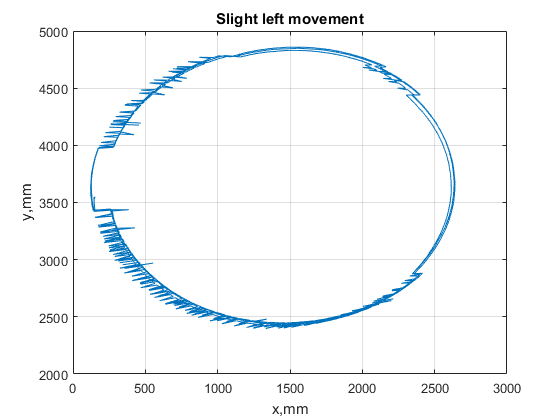
\includegraphics[scale = 0.8]{l.png}

  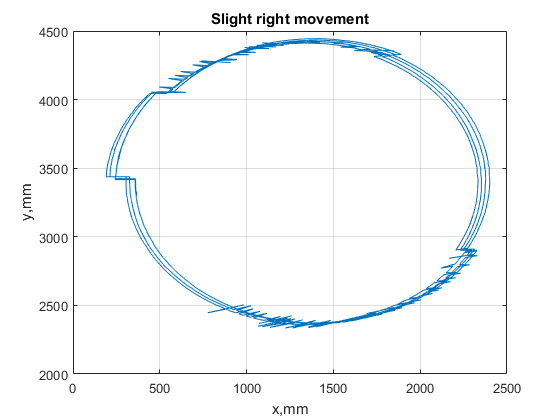
\includegraphics[scale = 0.8]{r.png}

  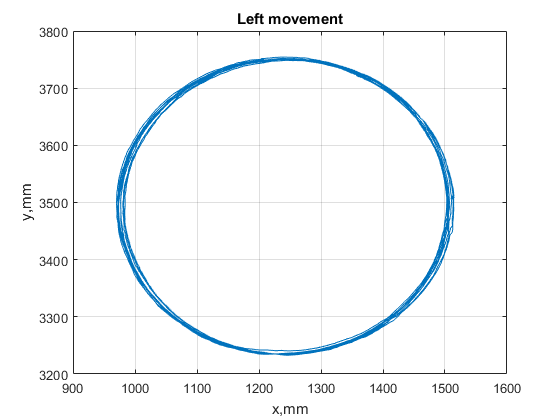
\includegraphics[scale = 0.8]{ll.png}

  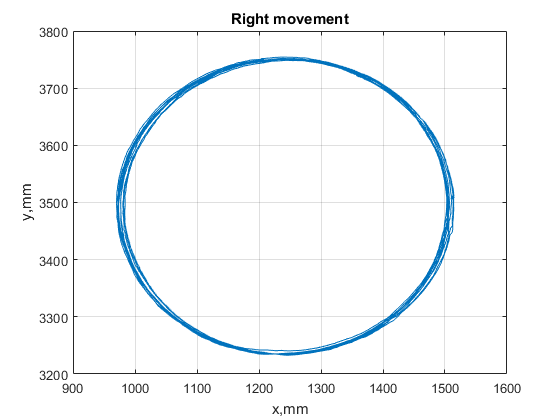
\includegraphics[scale = 0.8]{rr.png}
\end{center}

The results look in the following way:

\begin{lstlisting}
1477416993888 lifecam20 1510.82507324 3511.84960938 1.72770082951
1477416993936 lifecam20 1510.82507324 3511.84960938 1.72770082951
1477416994019 lifecam20 1511.18066406 3511.49462891 1.73569214344
1477416994210 lifecam20 1510.82507324 3511.84960938 1.72770082951
1477416994283 lifecam20 1510.86303711 3511.62670898 1.72653448582
...
\end{lstlisting}
where the first column is time, the second is a camera that is capturing the marker, third - x coordinate, forth - y coordinate and the last one is the robot's orientation. The results are in the attached excel files.

\section{Data processing}
If we want to find model parameters$\alpha_1 ...\alpha_4$ we need to process the data and it includes many steps.

\begin{itemize}
\item Remove noise when cameras switch.
\item Find real position of the robot instead of camera recorded position.
\item Chop recorded data into 40 separate movements and rotate final positions.
\item Use prediction model for unchopped data.
\end{itemize}
The implementation of parameter finding method are not clear right now, so this steps will be done after discussion.


\lstinputlisting{chop_data.m}

\section{Pose prediction}
The next pose of the robot can be predicted using previous pose, control command and time delay.

The code of pose prediction function:

\lstinputlisting{predict_pose.m}

\section{Pose prediction with linear relation}

In this case we assume that given commands are executed with some constant linear changes: $v_{effective} =k_v v+b_b $ , $\omega_{effective} =k_{\omega} v+b_{\omega} $. In order to find this linear coefficients, we can apply optimization procedure and use error function:

\begin{equation}
E = \sum\limits_i^N ||pose(i)_{predicted} - pose(i)_{true}||,
\end{equation}
where $N$ is number of sample positions.

Fitness function for finding linear coefficients for slight left movement:

\lstinputlisting{step2error.m}


This optimization can be done with command:
\begin{lstlisting}
  fminsearch(@step2error,[1,1,0,0])
\end{lstlisting}
That gave result: $[0.8568,    1.0490,    0.0003,   -0.0000]$. But after optimization the error is still high and it can be seen from the next figure that compares predicted path with real one:

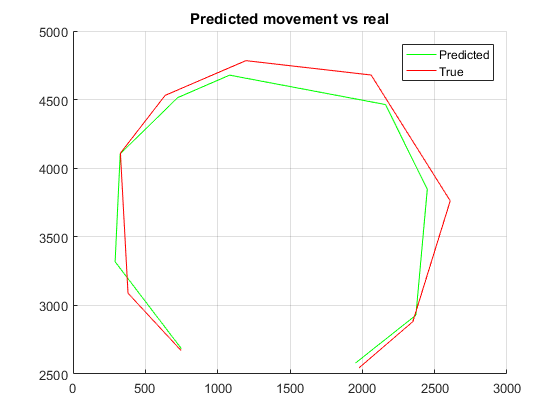
\includegraphics[scale = 1]{step2error.png}

It seems to be that linear relation is not enough for the motion model. We can increase number of training samples or change optimization method to reduce error within this model.


\section{Motion model parameter estimation}

The goal of this assignment is to create a motion model $x_t= f (x_{t-1} ,u_t ,\alpha_1, \alpha_2, \alpha_3, \alpha_4)$, where $u_t$ is a commanded $v, \omega$ motion and $x_t$ is the robot's pose,  by estimating its empirical parameters: $\alpha_1, \alpha_2, \alpha_3, \alpha_4$. We need to do it in such a way so it would have the same distribution that has a real robot's drive system.\\

The probability of robot's pose at the time t is the following:\\

$P(x_t |x{t-1}, u_t) = N(0, \alpha_1 v^2 + \alpha_2\omega^2) \cdot N (0, \alpha_3 v^2 + \alpha_4\omega^2)\cdot N (0, \alpha_5 v^2 + \alpha_5\omega^2)$,\\
where $v,\omega$ are linear and angular velocities respectively.\\

We are solving this problem as a problem of maximum likelihood estimation. We are maximizing a posterior $P(\alpha|X)$ using Bayes rule:\\

$P(\alpha|X) = \frac{P(\alpha|X)P(\alpha)}{P(X)}$\\

In our case this expression will take the following log-likelihood form:\\
$P(\alpha|X) = -\frac{1}{2}(3ln(2\pi) + ln(\alpha_1v^2 + \alpha2 \omega^2) + \frac{v - \hat{v}}{\alpha_1v^2 + \alpha2 \omega^2} + ln(\alpha_3v^2 + \alpha4 \omega^2) + \frac{\omega - \hat{\omega}}{\alpha_3v^2 + \alpha4 \omega^2})$\\

So, we can obtain the following derivatives:\\
$\frac{\partial P(\alpha|X)}{\partial \alpha_1} = -\frac{1}{2} (\frac{v^2}{\alpha_1v^2 + \alpha_2 \omega^2} - \frac{(v - \hat{v})v^2}{(\alpha_1v^2 + \alpha_2 \omega^2)^2})$\\
$\frac{\partial P(\alpha|X)}{\partial \alpha_2} = -\frac{1}{2} (\frac{\omega^2}{\alpha_1v^2 + \alpha_2 \omega^2} - \frac{(v - \hat{v})\omega^2}{(\alpha_1v^2 + \alpha_2 \omega^2)^2})$\\
$\frac{\partial P(\alpha|X)}{\partial \alpha_3} = -\frac{1}{2} (\frac{v^2}{\alpha_3v^2 + \alpha_4 \omega^2} - \frac{(\omega - \hat{\omega})v^2}{(\alpha_1v^3 + \alpha_4 \omega^2)^2})$\\
$\frac{\partial P(\alpha|X)}{\partial \alpha_4} = -\frac{1}{2} (\frac{\omega^2}{\alpha_3v^2 + \alpha_4 \omega^2} - \frac{(\omega - \hat{\omega})\omega^2}{(\alpha_1v^3 + \alpha_4 \omega^2)^2})$\\

It is important that we do not need $\alpha_5$ and $\alpha_6$, because we only calculate ...\\

X are independent, so:\\
$$\frac{\partial P(\alpha|X)}{\partial \alpha_j} = \sum_{i=1}^{n}\frac{\partial P(\alpha|x)}{\partial \alpha_j}$$\\
It can be solved as an optimization problem. We used the following Python code for $\alpha$s estimation:\\

\begin{lstlisting}
#!/usr/bin/env python3
import glob
import os
import numpy as np
from parameter_optimisation import optimise_parameters
import random

class Data(object):
    def __init__(self):
        self.trajectories = list()
        self.trajectories_end = list()
        self.time_deltas = list()
        pass

    pass


def read_data(directory_names):
    data_store = Data()
    for directory_name in directory_names:
        os.chdir(directory_name)
        trajectories = list()
        trajectories_end = list()
        times = list()

        files = list()
        for f in glob.glob("*.csv"):
            files.append(f)
            pass

        for f in files:
            data = np.loadtxt(f,delimiter=',')
            #data: shape(samples,4) -- [[time_stamp,x,y,gamma]]

            poses = np.zeros((data.shape[0], 3))
            time_deltas = np.zeros(data.shape[0]-1)

            poses[0,0] = 0.
            poses[0,1] = 0.
            poses[0,2] = 0.
            for i in range(1, data.shape[0]):
                poses[i,0] = data[i,1] - data[0,1]
                poses[i,1] = data[i,2] - data[0,2]
                poses[i,2] = data[i,3] - data[0,3]
                #time_deltas[i-1] = data[i,0] - data[i-1,0]
                time_deltas[i-1] = data[i,0] - data[0,0]
                pass

            trajectories.append(poses)
            trajectories_end.append(poses[-1])
            times.append(time_deltas)
            pass

        data_store.trajectories.append(trajectories)
        data_store.trajectories_end.append(trajectories_end)
        data_store.time_deltas.append(times)

        os.chdir('..')
        pass

    return data_store

def sample_gaussian(u, alphas):
    v_gaussian = random.normalvariate(0, alpha[0]*abs(u[0]) + alpha[1]*abs(u[1]))
    omega_gaussian = random.normalvariate(0, alpha[2]*abs(u[0]) + alpha[3]*abs(u[1]))
    gamma_gaussian = random.normalvariate(0, alpha[4]*abs(u[0]) + alpha[5]*abs(u[1]))
    return [v_gaussian, omega_gaussian, gamma_gaussian]

def motion_model_velocity(xt, ut, x_prevt, delta_t):
    mu = 0.5 * ((x_prevt[0] - xt[0]) * np.cos(x_prevt[2]) + (x_prevt[1] - xt[1]) * np.sin(x_prevt[2])) / ((x_prevt[1] - xt[1]) *
    np.cos(x_prevt[2]) - (x_prevt[0] - xt[0]) * np.sin(x_prevt[2]))
    x_star = 0.5 * (x_prevt[0] + xt[0]) + mu * (x_prevt[1] - xt[1])
    y_star = 0.5 * (x_prevt[1] + xt[1]) + mu * (xt[0] - x_prevt[0])
    r_star = np.sqrt((x_prevt[0] - x_star)**2 + (x_prevt[1] - y_star)**2)
    delta_theta = np.arctan2(xt[1] - y_star, xt[0] - x_star) - np.arctan2(x_prevt[1] - y_star, x_prevt[0] - x_star)
    v_hat = delta_theta / delta_t * r_star
    omega_hat = delta_theta / delta_t
    gamma_hat = (xt[2] - x_prevt[2]) / delta_t - omega_hat
    return np.array([ut[0], ut[1], v_hat, omega_hat, gamma_hat])


def sample_motion_model_velocity(u_current, pose_past, alpha, delta_t, sampled_gaussian = 0):
    """
    @param u_current: velocity command [v w]
    @param pose_past: pose [x y theta] at time step t-1
    @param alpha: 6-vector of the model's parameters
    @param delta_t: time difference between 2 time steps
    @param sampled_gaussian: pre-sampled guassian
    @return: pose [x y theta] at time step t
    """
    if (sampled_gaussian == 0):
        random.seed()
        v_hat = u_current[0] + random.normalvariate(0, alpha[0]*abs(u_current[0]) + alpha[1]*abs(u_current[1]))
        omega_hat = u_current[1] + random.normalvariate(0, alpha[2]*abs(u_current[0]) + alpha[3]*abs(u_current[1]))
        gamma_hat = random.normalvariate(0, alpha[4]*abs(u_current[0]) + alpha[5]*abs(u_current[1]))
    else:
        v_hat = u_current[0] + sampled_gaussian[0]
        omega_hat = u_current[1] + sampled_gaussian[1]
        gamma_hat = sampled_gaussian[2]

    x_current = (pose_past[0]
                 - v_hat/omega_hat*np.sin(pose_past[2])
                 + v_hat/omega_hat*np.sin(pose_past[2] + omega_hat*delta_t))

    y_current = (pose_past[1]
                 + v_hat/omega_hat*np.cos(pose_past[2])
                 - v_hat/omega_hat*np.cos(pose_past[2] + omega_hat*delta_t))

    theta_current = pose_past[2] + omega_hat*delta_t + gamma_hat*delta_t

    return (x_current, y_current, theta_current)

def predict_trajectory(u, pose_start, alpha, delta_t, duration, nb_experiment, single_gaussian = False):
    """
    @param u: velocity command [v w]
    @param pose_start: pose [x y theta] at time step t = 0
    @param alpha: 6-vector of the model's parameters
    @param delta_t: time difference between 2 time steps
    @param duration: running time
    @param nb_experiment: number of time the experiment is repeated
    @param single_gaussian: use single gaussian sample for each repeating exps
    @return: trajectory plot
    """
    n = int(duration/delta_t)
    trajectories = list()
    for i in range(nb_experiment):
        pose_current = pose_start
        poses = list()

        gaussian = 0

        if single_gaussian:
            gaussian = sample_gaussian(u, alpha)

        poses.append(pose_current)
        for j in range(n):
            pose_current = sample_motion_model_velocity(u, pose_current, alpha, delta_t, sampled_gaussian = gaussian)
            poses.append(pose_current)

        trajectories.append(poses)

    return np.array(trajectories)

def plot_trajectory(trajectories):
    for trajectory in trajectories:
        plt.plot(trajectory[:,0], trajectory[:,1])
    plt.show()

def plot_real_trajectories(data, nb_experiment):
    """
    @param data: data of shape [time, x, y, theta]
    @param nb_experiment: number of repeated experiments
    """
    nb_samples_per_experiment = int(len(data)/nb_experiment)

    trajectories = list()
    for i in range(nb_experiment):
        poses = list()

        poses.append([0, 0, 0])
        pose_start_index = i*nb_samples_per_experiment
        delta_theta = data[pose_start_index,3] - data[0,3]
        R = np.array([[np.cos(delta_theta), -np.sin(delta_theta)],
                       [np.sin(delta_theta),np.cos(delta_theta)]])
        for j in range(1,nb_samples_per_experiment):
            sample_index = i*nb_samples_per_experiment + j
            p = [0, 0, 0]
            p[0] = data[sample_index,1] - data[pose_start_index,1]
            p[1] = data[sample_index,2] - data[pose_start_index,2]
            p[2] = data[sample_index,3] - data[pose_start_index,3]
            poses.append(p)

        poses = np.array(poses)
        poses[:,:2] = np.dot(poses[:,:2],R)
        trajectories.append(poses)

    trajectories = np.array(trajectories)
    plot_trajectory(trajectories)


if __name__ == "__main__":
    #robot run time: 6.28s, 3.93s, 6.28s, 3.93s, 6.28s
    directory_names = ['straight', 'left', 'slight_left', 'right', 'slight_right']
    # speed is 100mm/s
    v = [100., 100., 100., 100., 100.]
    omega = [0., np.radians(22.92), np.radians(4.77), np.radians(-22.92), np.radians(-4.77)]
    data = read_data(directory_names)

    motion_model_data = list()
    for i, trajectories in enumerate(data.trajectories):
        for j, trajectory in enumerate(trajectories):
            for k in range(len(trajectory)-1):
                delta_t = data.time_deltas[i][j][k]
                #mmv = motion_model_velocity(trajectory[k+1], (v[i], omega[i]), trajectory[k], delta_t)
                mmv = motion_model_velocity(trajectory[k+1], (v[i], omega[i]), trajectory[0], delta_t)
                motion_model_data.append(mmv)
    motion_model_data = np.array(motion_model_data)


    init_alphas = np.random.uniform(1e-7, 1e-5, 6)
    alphas = optimise_parameters(motion_model_data, init_alphas)
    print(alphas)
    pass
\end{lstlisting}
\section{Parameter $\alpha$ estimation}

Optimization procedure is really sensitive to change of many parameters:
\begin{enumerate}
\item Very dense data (small difference between time steps) will cause divergence of the optimization method.
\item Initial $\alpha$ less that $10^{-1}$ will guarantee good coefficients.
\item  Initial $\alpha$ more that $10^{-1}$ will give coefficients that spoil motion prediction completely.
\item Commanded speed and angular speed can not be easily measured and this parameters spoil performance.
\end{enumerate}

 \medskip
 Good estimations of parameter $alpha$ are :$[ 0.0143,~    0.0478,~    0.0000 ,~   0.0662,~    0.0000 ,~   0.0804].$
 \medskip

 Example of bad parameters:  $[0.0143,~    2.2240,~    0.0000 ,~   0.1230 ,~   0.0000 ,~   1.4137]$


\section{Simulation results}

Motion model was started from one of the original points for around 1000 iterations (a few loops):

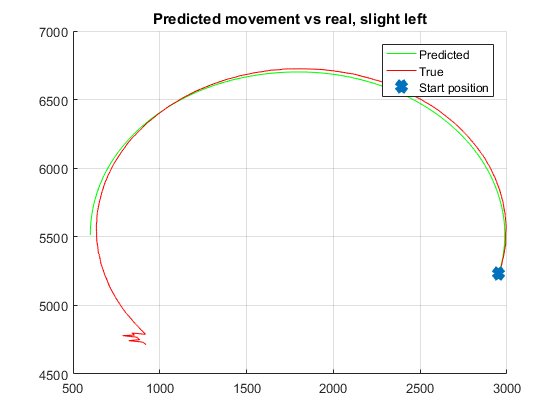
\includegraphics[scale = 1]{gl.png}

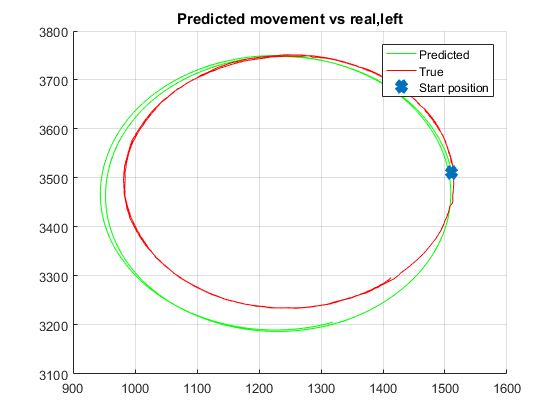
\includegraphics[scale = 1]{gll.png}

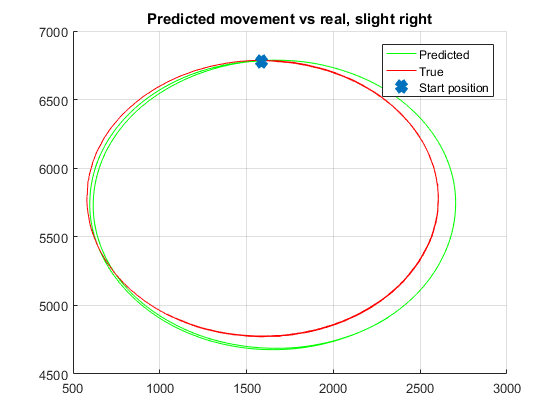
\includegraphics[scale = 1]{gr.png}

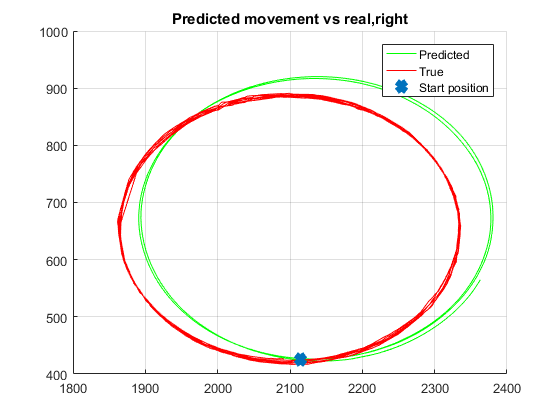
\includegraphics[scale = 1]{grr.png}

This results show that the main problem is not parameters $\alpha$ but good estimation of commanded speeds.

Bad set of parameters gave such results:

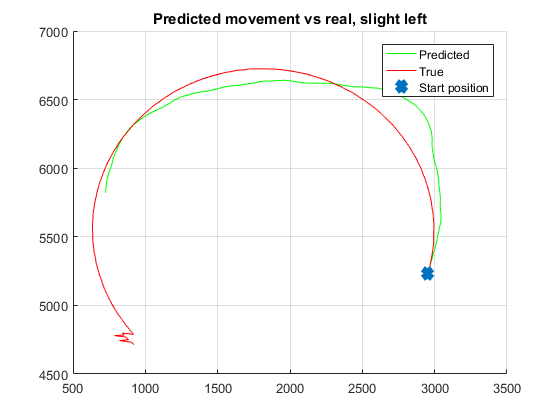
\includegraphics[scale = 1]{bl.png}

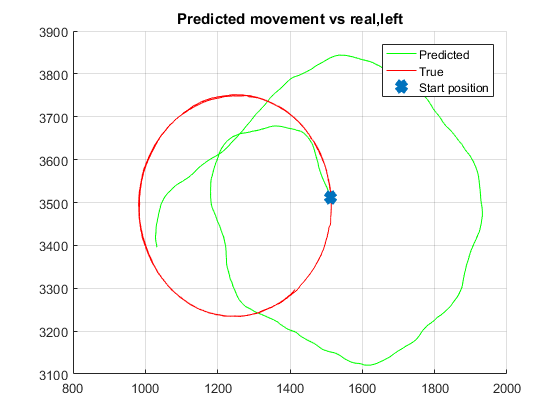
\includegraphics[scale = 1]{bll.png}

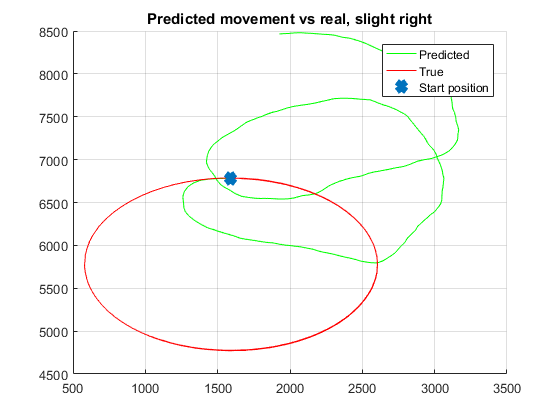
\includegraphics[scale = 1]{br.png}

As we can see, wrong alphas can spoil all motion prediction mechanism.


Multiple runs of one motion prediction sequence usually give bad precision because of wrong $v,\omega$ in simulation.

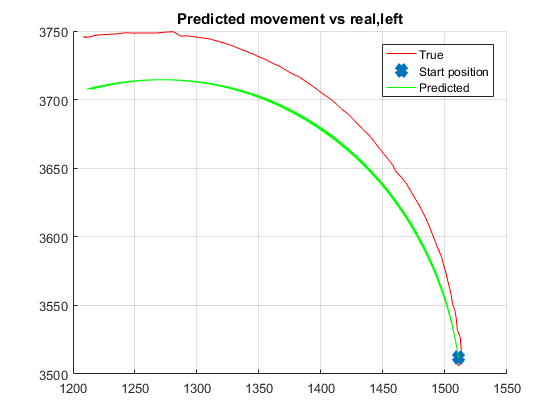
\includegraphics[scale = 1]{scatter.png}

\section{Conclusion}

Small circles show quite a good result, because the whole path can be covered by one camera. In large circles and straight motion we see some breaking points those most likely appeared because of camera switch. We tried to avoid it by using camera stitcher tool, but apparently it could't fix it completely. Usage of multiple markers might help, but in the Lego robot case the markers should be either very small that can make their detection hard or mounted on the large platform that may harm the robot's balance. To avoid this effect for a straight motion we've change an experiment so the robot would not cross the camera switching line.

\bigskip

Model parameter identification is multiple steps process and many steps have to be clarified. Now we can observe that linear motion prediction model works bad even after optimization. So, this model has to be changed to stochastic model.

\bigskip

But the main problem of finding good motion model is estimation of robot $v,\omega$. The ones we used from the commanded control give really biased results. So, there should be a better way to estimate this parameters.

\end{document}
